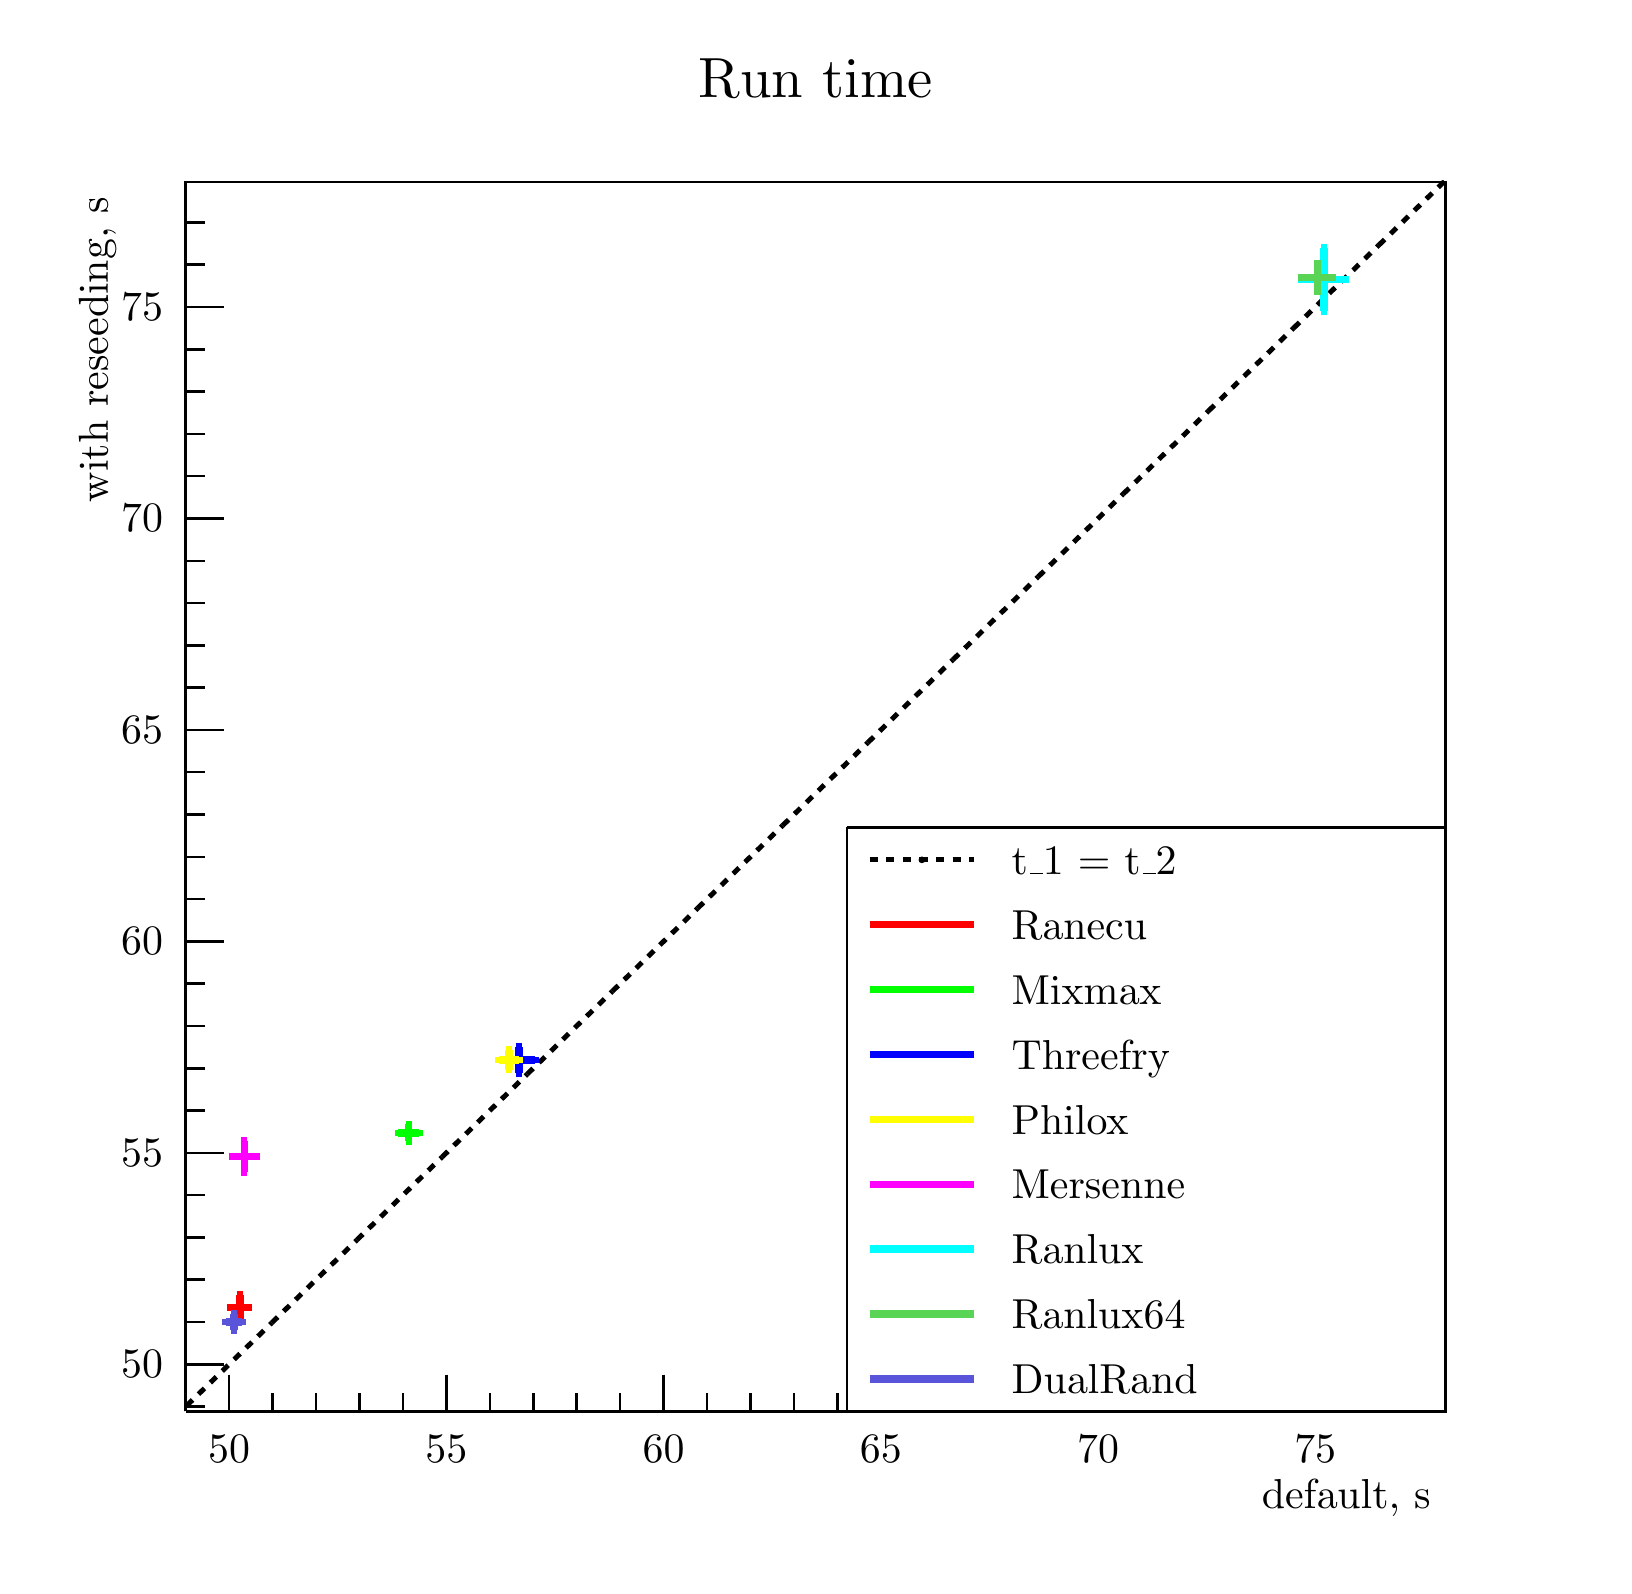
\begin{tikzpicture}
\pgfdeclareplotmark{cross} {
\pgfpathmoveto{\pgfpoint{-0.3\pgfplotmarksize}{\pgfplotmarksize}}
\pgfpathlineto{\pgfpoint{+0.3\pgfplotmarksize}{\pgfplotmarksize}}
\pgfpathlineto{\pgfpoint{+0.3\pgfplotmarksize}{0.3\pgfplotmarksize}}
\pgfpathlineto{\pgfpoint{+1\pgfplotmarksize}{0.3\pgfplotmarksize}}
\pgfpathlineto{\pgfpoint{+1\pgfplotmarksize}{-0.3\pgfplotmarksize}}
\pgfpathlineto{\pgfpoint{+0.3\pgfplotmarksize}{-0.3\pgfplotmarksize}}
\pgfpathlineto{\pgfpoint{+0.3\pgfplotmarksize}{-1.\pgfplotmarksize}}
\pgfpathlineto{\pgfpoint{-0.3\pgfplotmarksize}{-1.\pgfplotmarksize}}
\pgfpathlineto{\pgfpoint{-0.3\pgfplotmarksize}{-0.3\pgfplotmarksize}}
\pgfpathlineto{\pgfpoint{-1.\pgfplotmarksize}{-0.3\pgfplotmarksize}}
\pgfpathlineto{\pgfpoint{-1.\pgfplotmarksize}{0.3\pgfplotmarksize}}
\pgfpathlineto{\pgfpoint{-0.3\pgfplotmarksize}{0.3\pgfplotmarksize}}
\pgfpathclose
\pgfusepathqstroke
}
\pgfdeclareplotmark{cross*} {
\pgfpathmoveto{\pgfpoint{-0.3\pgfplotmarksize}{\pgfplotmarksize}}
\pgfpathlineto{\pgfpoint{+0.3\pgfplotmarksize}{\pgfplotmarksize}}
\pgfpathlineto{\pgfpoint{+0.3\pgfplotmarksize}{0.3\pgfplotmarksize}}
\pgfpathlineto{\pgfpoint{+1\pgfplotmarksize}{0.3\pgfplotmarksize}}
\pgfpathlineto{\pgfpoint{+1\pgfplotmarksize}{-0.3\pgfplotmarksize}}
\pgfpathlineto{\pgfpoint{+0.3\pgfplotmarksize}{-0.3\pgfplotmarksize}}
\pgfpathlineto{\pgfpoint{+0.3\pgfplotmarksize}{-1.\pgfplotmarksize}}
\pgfpathlineto{\pgfpoint{-0.3\pgfplotmarksize}{-1.\pgfplotmarksize}}
\pgfpathlineto{\pgfpoint{-0.3\pgfplotmarksize}{-0.3\pgfplotmarksize}}
\pgfpathlineto{\pgfpoint{-1.\pgfplotmarksize}{-0.3\pgfplotmarksize}}
\pgfpathlineto{\pgfpoint{-1.\pgfplotmarksize}{0.3\pgfplotmarksize}}
\pgfpathlineto{\pgfpoint{-0.3\pgfplotmarksize}{0.3\pgfplotmarksize}}
\pgfpathclose
\pgfusepathqfillstroke
}
\pgfdeclareplotmark{newstar} {
\pgfpathmoveto{\pgfqpoint{0pt}{\pgfplotmarksize}}
\pgfpathlineto{\pgfqpointpolar{44}{0.5\pgfplotmarksize}}
\pgfpathlineto{\pgfqpointpolar{18}{\pgfplotmarksize}}
\pgfpathlineto{\pgfqpointpolar{-20}{0.5\pgfplotmarksize}}
\pgfpathlineto{\pgfqpointpolar{-54}{\pgfplotmarksize}}
\pgfpathlineto{\pgfqpointpolar{-90}{0.5\pgfplotmarksize}}
\pgfpathlineto{\pgfqpointpolar{234}{\pgfplotmarksize}}
\pgfpathlineto{\pgfqpointpolar{198}{0.5\pgfplotmarksize}}
\pgfpathlineto{\pgfqpointpolar{162}{\pgfplotmarksize}}
\pgfpathlineto{\pgfqpointpolar{134}{0.5\pgfplotmarksize}}
\pgfpathclose
\pgfusepathqstroke
}
\pgfdeclareplotmark{newstar*} {
\pgfpathmoveto{\pgfqpoint{0pt}{\pgfplotmarksize}}
\pgfpathlineto{\pgfqpointpolar{44}{0.5\pgfplotmarksize}}
\pgfpathlineto{\pgfqpointpolar{18}{\pgfplotmarksize}}
\pgfpathlineto{\pgfqpointpolar{-20}{0.5\pgfplotmarksize}}
\pgfpathlineto{\pgfqpointpolar{-54}{\pgfplotmarksize}}
\pgfpathlineto{\pgfqpointpolar{-90}{0.5\pgfplotmarksize}}
\pgfpathlineto{\pgfqpointpolar{234}{\pgfplotmarksize}}
\pgfpathlineto{\pgfqpointpolar{198}{0.5\pgfplotmarksize}}
\pgfpathlineto{\pgfqpointpolar{162}{\pgfplotmarksize}}
\pgfpathlineto{\pgfqpointpolar{134}{0.5\pgfplotmarksize}}
\pgfpathclose
\pgfusepathqfillstroke
}
\definecolor{c}{rgb}{1,1,1};
\draw [color=c, fill=c] (0,0) rectangle (20,19.519);
\draw [color=c, fill=c] (2,1.9519) rectangle (18,17.5671);
\definecolor{c}{rgb}{0,0,0};
\draw [c,line width=0.9] (2,1.9519) -- (2,17.5671) -- (18,17.5671) -- (18,1.9519) -- (2,1.9519);
\definecolor{c}{rgb}{1,1,1};
\draw [color=c, fill=c] (2,1.9519) rectangle (18,17.5671);
\definecolor{c}{rgb}{0,0,0};
\draw [c,line width=0.9] (2,1.9519) -- (2,17.5671) -- (18,17.5671) -- (18,1.9519) -- (2,1.9519);
\draw [c,dashed,line width=1.8] (2.01103,2.02412) -- (2.0331,2.0456) -- (2.05517,2.06709) -- (2.07724,2.08857) -- (2.09931,2.11005) -- (2.12138,2.13154) -- (2.14345,2.15302) -- (2.16552,2.17451) -- (2.18759,2.19599) -- (2.20966,2.21747) --
 (2.23172,2.23896) -- (2.25379,2.26044) -- (2.27586,2.28193) -- (2.29793,2.30341) -- (2.32,2.3249) -- (2.34207,2.34638) -- (2.36414,2.36786) -- (2.38621,2.38935) -- (2.40828,2.41083) -- (2.43035,2.43232) -- (2.45241,2.4538) -- (2.47448,2.47528) --
 (2.49655,2.49677) -- (2.51862,2.51825) -- (2.54069,2.53974) -- (2.56276,2.56122) -- (2.58483,2.5827) -- (2.6069,2.60419) -- (2.62897,2.62567) -- (2.65103,2.64716) -- (2.6731,2.66864) -- (2.69517,2.69012) -- (2.71724,2.71161) -- (2.73931,2.73309) --
 (2.76138,2.75458) -- (2.78345,2.77606) -- (2.80552,2.79754) -- (2.82759,2.81903) -- (2.84966,2.84051) -- (2.87172,2.862) -- (2.89379,2.88348) -- (2.91586,2.90496) -- (2.93793,2.92645) -- (2.96,2.94793) -- (2.98207,2.96942) -- (3.00414,2.9909) --
 (3.02621,3.01238) -- (3.04828,3.03387) -- (3.07034,3.05535) -- (3.09241,3.07684);
\draw [c,dashed,line width=1.8] (3.09241,3.07684) -- (3.11448,3.09832) -- (3.13655,3.1198) -- (3.15862,3.14129) -- (3.18069,3.16277) -- (3.20276,3.18426) -- (3.22483,3.20574) -- (3.2469,3.22722) -- (3.26897,3.24871) -- (3.29103,3.27019) --
 (3.3131,3.29168) -- (3.33517,3.31316) -- (3.35724,3.33464) -- (3.37931,3.35613) -- (3.40138,3.37761) -- (3.42345,3.3991) -- (3.44552,3.42058) -- (3.46759,3.44206) -- (3.48966,3.46355) -- (3.51172,3.48503) -- (3.53379,3.50652) -- (3.55586,3.528) --
 (3.57793,3.54948) -- (3.6,3.57097) -- (3.62207,3.59245) -- (3.64414,3.61394) -- (3.66621,3.63542) -- (3.68828,3.6569) -- (3.71035,3.67839) -- (3.73241,3.69987) -- (3.75448,3.72136) -- (3.77655,3.74284) -- (3.79862,3.76432) -- (3.82069,3.78581) --
 (3.84276,3.80729) -- (3.86483,3.82878) -- (3.8869,3.85026) -- (3.90897,3.87174) -- (3.93103,3.89323) -- (3.9531,3.91471) -- (3.97517,3.9362) -- (3.99724,3.95768) -- (4.01931,3.97916) -- (4.04138,4.00065) -- (4.06345,4.02213) -- (4.08552,4.04362) --
 (4.10759,4.0651) -- (4.12966,4.08659) -- (4.15172,4.10807) -- (4.17379,4.12955);
\draw [c,dashed,line width=1.8] (4.17379,4.12955) -- (4.19586,4.15104) -- (4.21793,4.17252) -- (4.24,4.19401) -- (4.26207,4.21549) -- (4.28414,4.23697) -- (4.30621,4.25846) -- (4.32828,4.27994) -- (4.35035,4.30143) -- (4.37241,4.32291) --
 (4.39448,4.34439) -- (4.41655,4.36588) -- (4.43862,4.38736) -- (4.46069,4.40885) -- (4.48276,4.43033) -- (4.50483,4.45181) -- (4.5269,4.4733) -- (4.54897,4.49478) -- (4.57103,4.51627) -- (4.5931,4.53775) -- (4.61517,4.55923) -- (4.63724,4.58072) --
 (4.65931,4.6022) -- (4.68138,4.62369) -- (4.70345,4.64517) -- (4.72552,4.66665) -- (4.74759,4.68814) -- (4.76966,4.70962) -- (4.79172,4.73111) -- (4.81379,4.75259) -- (4.83586,4.77407) -- (4.85793,4.79556) -- (4.88,4.81704) -- (4.90207,4.83853) --
 (4.92414,4.86001) -- (4.94621,4.88149) -- (4.96828,4.90298) -- (4.99035,4.92446) -- (5.01241,4.94595) -- (5.03448,4.96743) -- (5.05655,4.98891) -- (5.07862,5.0104) -- (5.10069,5.03188) -- (5.12276,5.05337) -- (5.14483,5.07485) -- (5.1669,5.09633) --
 (5.18897,5.11782) -- (5.21103,5.1393) -- (5.2331,5.16079) -- (5.25517,5.18227);
\draw [c,dashed,line width=1.8] (5.25517,5.18227) -- (5.27724,5.20375) -- (5.29931,5.22524) -- (5.32138,5.24672) -- (5.34345,5.26821) -- (5.36552,5.28969) -- (5.38759,5.31117) -- (5.40966,5.33266) -- (5.43172,5.35414) -- (5.45379,5.37563) --
 (5.47586,5.39711) -- (5.49793,5.41859) -- (5.52,5.44008) -- (5.54207,5.46156) -- (5.56414,5.48305) -- (5.58621,5.50453) -- (5.60828,5.52601) -- (5.63034,5.5475) -- (5.65241,5.56898) -- (5.67448,5.59047) -- (5.69655,5.61195) -- (5.71862,5.63343) --
 (5.74069,5.65492) -- (5.76276,5.6764) -- (5.78483,5.69789) -- (5.8069,5.71937) -- (5.82897,5.74085) -- (5.85103,5.76234) -- (5.8731,5.78382) -- (5.89517,5.80531) -- (5.91724,5.82679) -- (5.93931,5.84828) -- (5.96138,5.86976) -- (5.98345,5.89124) --
 (6.00552,5.91273) -- (6.02759,5.93421) -- (6.04966,5.9557) -- (6.07172,5.97718) -- (6.09379,5.99866) -- (6.11586,6.02015) -- (6.13793,6.04163) -- (6.16,6.06312) -- (6.18207,6.0846) -- (6.20414,6.10608) -- (6.22621,6.12757) -- (6.24828,6.14905) --
 (6.27034,6.17054) -- (6.29241,6.19202) -- (6.31448,6.2135) -- (6.33655,6.23499);
\draw [c,dashed,line width=1.8] (6.33655,6.23499) -- (6.35862,6.25647) -- (6.38069,6.27796) -- (6.40276,6.29944) -- (6.42483,6.32092) -- (6.4469,6.34241) -- (6.46897,6.36389) -- (6.49103,6.38538) -- (6.5131,6.40686) -- (6.53517,6.42834) --
 (6.55724,6.44983) -- (6.57931,6.47131) -- (6.60138,6.4928) -- (6.62345,6.51428) -- (6.64552,6.53576) -- (6.66759,6.55725) -- (6.68966,6.57873) -- (6.71172,6.60022) -- (6.73379,6.6217) -- (6.75586,6.64318) -- (6.77793,6.66467) -- (6.8,6.68615) --
 (6.82207,6.70764) -- (6.84414,6.72912) -- (6.86621,6.7506) -- (6.88828,6.77209) -- (6.91035,6.79357) -- (6.93241,6.81506) -- (6.95448,6.83654) -- (6.97655,6.85802) -- (6.99862,6.87951) -- (7.02069,6.90099) -- (7.04276,6.92248) -- (7.06483,6.94396)
 -- (7.0869,6.96544) -- (7.10897,6.98693) -- (7.13103,7.00841) -- (7.1531,7.0299) -- (7.17517,7.05138) -- (7.19724,7.07286) -- (7.21931,7.09435) -- (7.24138,7.11583) -- (7.26345,7.13732) -- (7.28552,7.1588) -- (7.30759,7.18028) -- (7.32966,7.20177)
 -- (7.35172,7.22325) -- (7.37379,7.24474) -- (7.39586,7.26622) -- (7.41793,7.2877);
\draw [c,dashed,line width=1.8] (7.41793,7.2877) -- (7.44,7.30919) -- (7.46207,7.33067) -- (7.48414,7.35216) -- (7.50621,7.37364) -- (7.52828,7.39512) -- (7.55034,7.41661) -- (7.57241,7.43809) -- (7.59448,7.45958) -- (7.61655,7.48106) --
 (7.63862,7.50254) -- (7.66069,7.52403) -- (7.68276,7.54551) -- (7.70483,7.567) -- (7.7269,7.58848) -- (7.74897,7.60997) -- (7.77103,7.63145) -- (7.7931,7.65293) -- (7.81517,7.67442) -- (7.83724,7.6959) -- (7.85931,7.71739) -- (7.88138,7.73887) --
 (7.90345,7.76035) -- (7.92552,7.78184) -- (7.94759,7.80332) -- (7.96966,7.82481) -- (7.99172,7.84629) -- (8.01379,7.86777) -- (8.03586,7.88926) -- (8.05793,7.91074) -- (8.08,7.93223) -- (8.10207,7.95371) -- (8.12414,7.97519) -- (8.14621,7.99668) --
 (8.16828,8.01816) -- (8.19034,8.03965) -- (8.21241,8.06113) -- (8.23448,8.08261) -- (8.25655,8.1041) -- (8.27862,8.12558) -- (8.30069,8.14707) -- (8.32276,8.16855) -- (8.34483,8.19003) -- (8.3669,8.21152) -- (8.38897,8.233) -- (8.41103,8.25449) --
 (8.4331,8.27597) -- (8.45517,8.29745) -- (8.47724,8.31894) -- (8.49931,8.34042);
\draw [c,dashed,line width=1.8] (8.49931,8.34042) -- (8.52138,8.36191) -- (8.54345,8.38339) -- (8.56552,8.40487) -- (8.58759,8.42636) -- (8.60966,8.44784) -- (8.63172,8.46933) -- (8.65379,8.49081) -- (8.67586,8.51229) -- (8.69793,8.53378) --
 (8.72,8.55526) -- (8.74207,8.57675) -- (8.76414,8.59823) -- (8.78621,8.61971) -- (8.80828,8.6412) -- (8.83035,8.66268) -- (8.85241,8.68417) -- (8.87448,8.70565) -- (8.89655,8.72713) -- (8.91862,8.74862) -- (8.94069,8.7701) -- (8.96276,8.79159) --
 (8.98483,8.81307) -- (9.0069,8.83455) -- (9.02897,8.85604) -- (9.05103,8.87752) -- (9.0731,8.89901) -- (9.09517,8.92049) -- (9.11724,8.94197) -- (9.13931,8.96346) -- (9.16138,8.98494) -- (9.18345,9.00643) -- (9.20552,9.02791) -- (9.22759,9.04939) --
 (9.24965,9.07088) -- (9.27172,9.09236) -- (9.29379,9.11385) -- (9.31586,9.13533) -- (9.33793,9.15681) -- (9.36,9.1783) -- (9.38207,9.19978) -- (9.40414,9.22127) -- (9.42621,9.24275) -- (9.44828,9.26423) -- (9.47034,9.28572) -- (9.49241,9.3072) --
 (9.51448,9.32869) -- (9.53655,9.35017) -- (9.55862,9.37166) -- (9.58069,9.39314);
\draw [c,dashed,line width=1.8] (9.58069,9.39314) -- (9.60276,9.41462) -- (9.62483,9.43611) -- (9.6469,9.45759) -- (9.66897,9.47908) -- (9.69103,9.50056) -- (9.7131,9.52204) -- (9.73517,9.54353) -- (9.75724,9.56501) -- (9.77931,9.5865) --
 (9.80138,9.60798) -- (9.82345,9.62946) -- (9.84552,9.65095) -- (9.86759,9.67243) -- (9.88966,9.69392) -- (9.91172,9.7154) -- (9.93379,9.73688) -- (9.95586,9.75837) -- (9.97793,9.77985) -- (10,9.80134) -- (10.0221,9.82282) -- (10.0441,9.8443) --
 (10.0662,9.86579) -- (10.0883,9.88727) -- (10.1103,9.90876) -- (10.1324,9.93024) -- (10.1545,9.95172) -- (10.1766,9.97321) -- (10.1986,9.99469) -- (10.2207,10.0162) -- (10.2428,10.0377) -- (10.2648,10.0591) -- (10.2869,10.0806) -- (10.309,10.1021)
 -- (10.331,10.1236) -- (10.3531,10.1451) -- (10.3752,10.1666) -- (10.3972,10.188) -- (10.4193,10.2095) -- (10.4414,10.231) -- (10.4634,10.2525) -- (10.4855,10.274) -- (10.5076,10.2955) -- (10.5297,10.317) -- (10.5517,10.3384) -- (10.5738,10.3599) --
 (10.5959,10.3814) -- (10.6179,10.4029) -- (10.64,10.4244) -- (10.6621,10.4459);
\draw [c,dashed,line width=1.8] (10.6621,10.4459) -- (10.6841,10.4673) -- (10.7062,10.4888) -- (10.7283,10.5103) -- (10.7503,10.5318) -- (10.7724,10.5533) -- (10.7945,10.5748) -- (10.8166,10.5962) -- (10.8386,10.6177) -- (10.8607,10.6392) --
 (10.8828,10.6607) -- (10.9048,10.6822) -- (10.9269,10.7037) -- (10.949,10.7251) -- (10.971,10.7466) -- (10.9931,10.7681) -- (11.0152,10.7896) -- (11.0372,10.8111) -- (11.0593,10.8326) -- (11.0814,10.8541) -- (11.1034,10.8755) -- (11.1255,10.897) --
 (11.1476,10.9185) -- (11.1697,10.94) -- (11.1917,10.9615) -- (11.2138,10.983) -- (11.2359,11.0044) -- (11.2579,11.0259) -- (11.28,11.0474) -- (11.3021,11.0689) -- (11.3241,11.0904) -- (11.3462,11.1119) -- (11.3683,11.1333) -- (11.3903,11.1548) --
 (11.4124,11.1763) -- (11.4345,11.1978) -- (11.4566,11.2193) -- (11.4786,11.2408) -- (11.5007,11.2622) -- (11.5228,11.2837) -- (11.5448,11.3052) -- (11.5669,11.3267) -- (11.589,11.3482) -- (11.611,11.3697) -- (11.6331,11.3912) -- (11.6552,11.4126) --
 (11.6772,11.4341) -- (11.6993,11.4556) -- (11.7214,11.4771) -- (11.7434,11.4986);
\draw [c,dashed,line width=1.8] (11.7434,11.4986) -- (11.7655,11.5201) -- (11.7876,11.5415) -- (11.8097,11.563) -- (11.8317,11.5845) -- (11.8538,11.606) -- (11.8759,11.6275) -- (11.8979,11.649) -- (11.92,11.6704) -- (11.9421,11.6919) --
 (11.9641,11.7134) -- (11.9862,11.7349) -- (12.0083,11.7564) -- (12.0303,11.7779) -- (12.0524,11.7993) -- (12.0745,11.8208) -- (12.0966,11.8423) -- (12.1186,11.8638) -- (12.1407,11.8853) -- (12.1628,11.9068) -- (12.1848,11.9283) -- (12.2069,11.9497)
 -- (12.229,11.9712) -- (12.251,11.9927) -- (12.2731,12.0142) -- (12.2952,12.0357) -- (12.3172,12.0572) -- (12.3393,12.0786) -- (12.3614,12.1001) -- (12.3834,12.1216) -- (12.4055,12.1431) -- (12.4276,12.1646) -- (12.4497,12.1861) -- (12.4717,12.2075)
 -- (12.4938,12.229) -- (12.5159,12.2505) -- (12.5379,12.272) -- (12.56,12.2935) -- (12.5821,12.315) -- (12.6041,12.3365) -- (12.6262,12.3579) -- (12.6483,12.3794) -- (12.6703,12.4009) -- (12.6924,12.4224) -- (12.7145,12.4439) -- (12.7366,12.4654) --
 (12.7586,12.4868) -- (12.7807,12.5083) -- (12.8028,12.5298) -- (12.8248,12.5513);
\draw [c,dashed,line width=1.8] (12.8248,12.5513) -- (12.8469,12.5728) -- (12.869,12.5943) -- (12.891,12.6157) -- (12.9131,12.6372) -- (12.9352,12.6587) -- (12.9572,12.6802) -- (12.9793,12.7017) -- (13.0014,12.7232) -- (13.0234,12.7446) --
 (13.0455,12.7661) -- (13.0676,12.7876) -- (13.0897,12.8091) -- (13.1117,12.8306) -- (13.1338,12.8521) -- (13.1559,12.8736) -- (13.1779,12.895) -- (13.2,12.9165) -- (13.2221,12.938) -- (13.2441,12.9595) -- (13.2662,12.981) -- (13.2883,13.0025) --
 (13.3103,13.0239) -- (13.3324,13.0454) -- (13.3545,13.0669) -- (13.3766,13.0884) -- (13.3986,13.1099) -- (13.4207,13.1314) -- (13.4428,13.1528) -- (13.4648,13.1743) -- (13.4869,13.1958) -- (13.509,13.2173) -- (13.531,13.2388) -- (13.5531,13.2603) --
 (13.5752,13.2817) -- (13.5972,13.3032) -- (13.6193,13.3247) -- (13.6414,13.3462) -- (13.6634,13.3677) -- (13.6855,13.3892) -- (13.7076,13.4107) -- (13.7297,13.4321) -- (13.7517,13.4536) -- (13.7738,13.4751) -- (13.7959,13.4966) -- (13.8179,13.5181)
 -- (13.84,13.5396) -- (13.8621,13.561) -- (13.8841,13.5825) -- (13.9062,13.604);
\draw [c,dashed,line width=1.8] (13.9062,13.604) -- (13.9283,13.6255) -- (13.9503,13.647) -- (13.9724,13.6685) -- (13.9945,13.6899) -- (14.0166,13.7114) -- (14.0386,13.7329) -- (14.0607,13.7544) -- (14.0828,13.7759) -- (14.1048,13.7974) --
 (14.1269,13.8188) -- (14.149,13.8403) -- (14.171,13.8618) -- (14.1931,13.8833) -- (14.2152,13.9048) -- (14.2372,13.9263) -- (14.2593,13.9478) -- (14.2814,13.9692) -- (14.3034,13.9907) -- (14.3255,14.0122) -- (14.3476,14.0337) -- (14.3697,14.0552) --
 (14.3917,14.0767) -- (14.4138,14.0981) -- (14.4359,14.1196) -- (14.4579,14.1411) -- (14.48,14.1626) -- (14.5021,14.1841) -- (14.5241,14.2056) -- (14.5462,14.227) -- (14.5683,14.2485) -- (14.5903,14.27) -- (14.6124,14.2915) -- (14.6345,14.313) --
 (14.6566,14.3345) -- (14.6786,14.3559) -- (14.7007,14.3774) -- (14.7228,14.3989) -- (14.7448,14.4204) -- (14.7669,14.4419) -- (14.789,14.4634) -- (14.811,14.4849) -- (14.8331,14.5063) -- (14.8552,14.5278) -- (14.8772,14.5493) -- (14.8993,14.5708) --
 (14.9214,14.5923) -- (14.9434,14.6138) -- (14.9655,14.6352) -- (14.9876,14.6567);
\draw [c,dashed,line width=1.8] (14.9876,14.6567) -- (15.0097,14.6782) -- (15.0317,14.6997) -- (15.0538,14.7212) -- (15.0759,14.7427) -- (15.0979,14.7641) -- (15.12,14.7856) -- (15.1421,14.8071) -- (15.1641,14.8286) -- (15.1862,14.8501) --
 (15.2083,14.8716) -- (15.2303,14.893) -- (15.2524,14.9145) -- (15.2745,14.936) -- (15.2966,14.9575) -- (15.3186,14.979) -- (15.3407,15.0005) -- (15.3628,15.022) -- (15.3848,15.0434) -- (15.4069,15.0649) -- (15.429,15.0864) -- (15.451,15.1079) --
 (15.4731,15.1294) -- (15.4952,15.1509) -- (15.5172,15.1723) -- (15.5393,15.1938) -- (15.5614,15.2153) -- (15.5834,15.2368) -- (15.6055,15.2583) -- (15.6276,15.2798) -- (15.6497,15.3012) -- (15.6717,15.3227) -- (15.6938,15.3442) -- (15.7159,15.3657)
 -- (15.7379,15.3872) -- (15.76,15.4087) -- (15.7821,15.4302) -- (15.8041,15.4516) -- (15.8262,15.4731) -- (15.8483,15.4946) -- (15.8703,15.5161) -- (15.8924,15.5376) -- (15.9145,15.5591) -- (15.9366,15.5805) -- (15.9586,15.602) -- (15.9807,15.6235)
 -- (16.0028,15.645) -- (16.0248,15.6665) -- (16.0469,15.688) -- (16.069,15.7094);
\draw [c,dashed,line width=1.8] (16.069,15.7094) -- (16.091,15.7309) -- (16.1131,15.7524) -- (16.1352,15.7739) -- (16.1572,15.7954) -- (16.1793,15.8169) -- (16.2014,15.8383) -- (16.2234,15.8598) -- (16.2455,15.8813) -- (16.2676,15.9028) --
 (16.2897,15.9243) -- (16.3117,15.9458) -- (16.3338,15.9673) -- (16.3559,15.9887) -- (16.3779,16.0102) -- (16.4,16.0317) -- (16.4221,16.0532) -- (16.4441,16.0747) -- (16.4662,16.0962) -- (16.4883,16.1176) -- (16.5103,16.1391) -- (16.5324,16.1606) --
 (16.5545,16.1821) -- (16.5766,16.2036) -- (16.5986,16.2251) -- (16.6207,16.2465) -- (16.6428,16.268) -- (16.6648,16.2895) -- (16.6869,16.311) -- (16.709,16.3325) -- (16.731,16.354) -- (16.7531,16.3754) -- (16.7752,16.3969) -- (16.7972,16.4184) --
 (16.8193,16.4399) -- (16.8414,16.4614) -- (16.8634,16.4829) -- (16.8855,16.5044) -- (16.9076,16.5258) -- (16.9297,16.5473) -- (16.9517,16.5688) -- (16.9738,16.5903) -- (16.9959,16.6118) -- (17.0179,16.6333) -- (17.04,16.6547) -- (17.0621,16.6762) --
 (17.0841,16.6977) -- (17.1062,16.7192) -- (17.1283,16.7407) -- (17.1503,16.7622);
\draw [c,dashed,line width=1.8] (17.1503,16.7622) -- (17.1724,16.7836) -- (17.1945,16.8051) -- (17.2166,16.8266) -- (17.2386,16.8481) -- (17.2607,16.8696) -- (17.2828,16.8911) -- (17.3048,16.9125) -- (17.3269,16.934) -- (17.349,16.9555) --
 (17.371,16.977) -- (17.3931,16.9985) -- (17.4152,17.02) -- (17.4372,17.0415) -- (17.4593,17.0629) -- (17.4814,17.0844) -- (17.5034,17.1059) -- (17.5255,17.1274) -- (17.5476,17.1489) -- (17.5697,17.1704) -- (17.5917,17.1918) -- (17.6138,17.2133) --
 (17.6359,17.2348) -- (17.6579,17.2563) -- (17.68,17.2778) -- (17.7021,17.2993) -- (17.7241,17.3207) -- (17.7462,17.3422) -- (17.7683,17.3637) -- (17.7903,17.3852) -- (17.8124,17.4067) -- (17.8345,17.4282) -- (17.8566,17.4496) -- (17.8786,17.4711) --
 (17.9007,17.4926) -- (17.9228,17.5141) -- (17.9448,17.5356) -- (17.9669,17.5571) -- (17.989,17.5671);
\draw [c,line width=0.9] (2,1.9519) -- (18,1.9519);
\draw [anchor= east] (18,0.858838) node[scale=1.51329, color=c, rotate=0]{default, s};
\draw [c,line width=0.9] (2.55172,2.42036) -- (2.55172,1.9519);
\draw [c,line width=0.9] (3.10345,2.18613) -- (3.10345,1.9519);
\draw [c,line width=0.9] (3.65517,2.18613) -- (3.65517,1.9519);
\draw [c,line width=0.9] (4.2069,2.18613) -- (4.2069,1.9519);
\draw [c,line width=0.9] (4.75862,2.18613) -- (4.75862,1.9519);
\draw [c,line width=0.9] (5.31034,2.42036) -- (5.31034,1.9519);
\draw [c,line width=0.9] (5.86207,2.18613) -- (5.86207,1.9519);
\draw [c,line width=0.9] (6.41379,2.18613) -- (6.41379,1.9519);
\draw [c,line width=0.9] (6.96552,2.18613) -- (6.96552,1.9519);
\draw [c,line width=0.9] (7.51724,2.18613) -- (7.51724,1.9519);
\draw [c,line width=0.9] (8.06897,2.42036) -- (8.06897,1.9519);
\draw [c,line width=0.9] (8.62069,2.18613) -- (8.62069,1.9519);
\draw [c,line width=0.9] (9.17241,2.18613) -- (9.17241,1.9519);
\draw [c,line width=0.9] (9.72414,2.18613) -- (9.72414,1.9519);
\draw [c,line width=0.9] (10.2759,2.18613) -- (10.2759,1.9519);
\draw [c,line width=0.9] (10.8276,2.42036) -- (10.8276,1.9519);
\draw [c,line width=0.9] (11.3793,2.18613) -- (11.3793,1.9519);
\draw [c,line width=0.9] (11.931,2.18613) -- (11.931,1.9519);
\draw [c,line width=0.9] (12.4828,2.18613) -- (12.4828,1.9519);
\draw [c,line width=0.9] (13.0345,2.18613) -- (13.0345,1.9519);
\draw [c,line width=0.9] (13.5862,2.42036) -- (13.5862,1.9519);
\draw [c,line width=0.9] (14.1379,2.18613) -- (14.1379,1.9519);
\draw [c,line width=0.9] (14.6897,2.18613) -- (14.6897,1.9519);
\draw [c,line width=0.9] (15.2414,2.18613) -- (15.2414,1.9519);
\draw [c,line width=0.9] (15.7931,2.18613) -- (15.7931,1.9519);
\draw [c,line width=0.9] (16.3448,2.42036) -- (16.3448,1.9519);
\draw [c,line width=0.9] (2.55172,2.42036) -- (2.55172,1.9519);
\draw [c,line width=0.9] (2,2.18613) -- (2,1.9519);
\draw [c,line width=0.9] (16.3448,2.42036) -- (16.3448,1.9519);
\draw [c,line width=0.9] (16.8966,2.18613) -- (16.8966,1.9519);
\draw [c,line width=0.9] (17.4483,2.18613) -- (17.4483,1.9519);
\draw [c,line width=0.9] (18,2.18613) -- (18,1.9519);
\draw [anchor=base] (2.55172,1.30778) node[scale=1.51329, color=c, rotate=0]{50};
\draw [anchor=base] (5.31034,1.30778) node[scale=1.51329, color=c, rotate=0]{55};
\draw [anchor=base] (8.06897,1.30778) node[scale=1.51329, color=c, rotate=0]{60};
\draw [anchor=base] (10.8276,1.30778) node[scale=1.51329, color=c, rotate=0]{65};
\draw [anchor=base] (13.5862,1.30778) node[scale=1.51329, color=c, rotate=0]{70};
\draw [anchor=base] (16.3448,1.30778) node[scale=1.51329, color=c, rotate=0]{75};
\draw [c,line width=0.9] (2,1.9519) -- (2,17.5671);
\draw [anchor= east] (0.88,17.5671) node[scale=1.51329, color=c, rotate=90]{with reseeding, s};
\draw [c,line width=0.9] (2.48,2.55048) -- (2,2.55048);
\draw [c,line width=0.9] (2.24,3.08758) -- (2,3.08758);
\draw [c,line width=0.9] (2.24,3.62468) -- (2,3.62468);
\draw [c,line width=0.9] (2.24,4.16178) -- (2,4.16178);
\draw [c,line width=0.9] (2.24,4.69888) -- (2,4.69888);
\draw [c,line width=0.9] (2.48,5.23598) -- (2,5.23598);
\draw [c,line width=0.9] (2.24,5.77308) -- (2,5.77308);
\draw [c,line width=0.9] (2.24,6.31018) -- (2,6.31018);
\draw [c,line width=0.9] (2.24,6.84728) -- (2,6.84728);
\draw [c,line width=0.9] (2.24,7.38438) -- (2,7.38438);
\draw [c,line width=0.9] (2.48,7.92148) -- (2,7.92148);
\draw [c,line width=0.9] (2.24,8.45858) -- (2,8.45858);
\draw [c,line width=0.9] (2.24,8.99568) -- (2,8.99568);
\draw [c,line width=0.9] (2.24,9.53279) -- (2,9.53279);
\draw [c,line width=0.9] (2.24,10.0699) -- (2,10.0699);
\draw [c,line width=0.9] (2.48,10.607) -- (2,10.607);
\draw [c,line width=0.9] (2.24,11.1441) -- (2,11.1441);
\draw [c,line width=0.9] (2.24,11.6812) -- (2,11.6812);
\draw [c,line width=0.9] (2.24,12.2183) -- (2,12.2183);
\draw [c,line width=0.9] (2.24,12.7554) -- (2,12.7554);
\draw [c,line width=0.9] (2.48,13.2925) -- (2,13.2925);
\draw [c,line width=0.9] (2.24,13.8296) -- (2,13.8296);
\draw [c,line width=0.9] (2.24,14.3667) -- (2,14.3667);
\draw [c,line width=0.9] (2.24,14.9038) -- (2,14.9038);
\draw [c,line width=0.9] (2.24,15.4409) -- (2,15.4409);
\draw [c,line width=0.9] (2.48,15.978) -- (2,15.978);
\draw [c,line width=0.9] (2.48,2.55048) -- (2,2.55048);
\draw [c,line width=0.9] (2.24,2.01338) -- (2,2.01338);
\draw [c,line width=0.9] (2.48,15.978) -- (2,15.978);
\draw [c,line width=0.9] (2.24,16.5151) -- (2,16.5151);
\draw [c,line width=0.9] (2.24,17.0522) -- (2,17.0522);
\draw [anchor= east] (1.9,2.55048) node[scale=1.51329, color=c, rotate=0]{50};
\draw [anchor= east] (1.9,5.23598) node[scale=1.51329, color=c, rotate=0]{55};
\draw [anchor= east] (1.9,7.92148) node[scale=1.51329, color=c, rotate=0]{60};
\draw [anchor= east] (1.9,10.607) node[scale=1.51329, color=c, rotate=0]{65};
\draw [anchor= east] (1.9,13.2925) node[scale=1.51329, color=c, rotate=0]{70};
\draw [anchor= east] (1.9,15.978) node[scale=1.51329, color=c, rotate=0]{75};
\definecolor{c}{rgb}{1,0,0};
\draw [c,line width=2.7] (2.68745,3.27234) -- (2.576,3.27234);
\draw [c,line width=2.7] (2.576,3.23226) -- (2.576,3.31242);
\draw [c,line width=2.7] (2.68745,3.27234) -- (2.7989,3.27234);
\draw [c,line width=2.7] (2.7989,3.23226) -- (2.7989,3.31242);
\draw [c,line width=2.7] (2.68745,3.27234) -- (2.68745,3.42917);
\draw [c,line width=2.7] (2.64737,3.42917) -- (2.72753,3.42917);
\draw [c,line width=2.7] (2.68745,3.27234) -- (2.68745,3.11551);
\draw [c,line width=2.7] (2.64737,3.11551) -- (2.72753,3.11551);
\foreach \P in {(2.68745,3.27234)}{\draw[mark options={color=c,fill=c},mark size=2.402402pt,mark=*,mark size=1pt] plot coordinates {\P};}
\definecolor{c}{rgb}{0,1,0};
\draw [c,line width=2.7] (4.832,5.49003) -- (4.69959,5.49003);
\draw [c,line width=2.7] (4.69959,5.44995) -- (4.69959,5.53011);
\draw [c,line width=2.7] (4.832,5.49003) -- (4.96441,5.49003);
\draw [c,line width=2.7] (4.96441,5.44995) -- (4.96441,5.53011);
\draw [c,line width=2.7] (4.832,5.49003) -- (4.832,5.59852);
\draw [c,line width=2.7] (4.79192,5.59852) -- (4.87208,5.59852);
\draw [c,line width=2.7] (4.832,5.49003) -- (4.832,5.38153);
\draw [c,line width=2.7] (4.79192,5.38153) -- (4.87208,5.38153);
\foreach \P in {(4.832,5.49003)}{\draw[mark options={color=c,fill=c},mark size=2.402402pt,mark=*,mark size=1pt] plot coordinates {\P};}
\definecolor{c}{rgb}{0,0,1};
\draw [c,line width=2.7] (6.23117,6.41653) -- (6.02538,6.41653);
\draw [c,line width=2.7] (6.02538,6.37645) -- (6.02538,6.45661);
\draw [c,line width=2.7] (6.23117,6.41653) -- (6.43697,6.41653);
\draw [c,line width=2.7] (6.43697,6.37645) -- (6.43697,6.45661);
\draw [c,line width=2.7] (6.23117,6.41653) -- (6.23117,6.58303);
\draw [c,line width=2.7] (6.19109,6.58303) -- (6.27125,6.58303);
\draw [c,line width=2.7] (6.23117,6.41653) -- (6.23117,6.25003);
\draw [c,line width=2.7] (6.19109,6.25003) -- (6.27125,6.25003);
\foreach \P in {(6.23117,6.41653)}{\draw[mark options={color=c,fill=c},mark size=2.402402pt,mark=*,mark size=1pt] plot coordinates {\P};}
\definecolor{c}{rgb}{1,1,0};
\draw [c,line width=2.7] (6.10538,6.41814) -- (5.97628,6.41814);
\draw [c,line width=2.7] (5.97628,6.37806) -- (5.97628,6.45822);
\draw [c,line width=2.7] (6.10538,6.41814) -- (6.23448,6.41814);
\draw [c,line width=2.7] (6.23448,6.37806) -- (6.23448,6.45822);
\draw [c,line width=2.7] (6.10538,6.41814) -- (6.10538,6.54436);
\draw [c,line width=2.7] (6.0653,6.54436) -- (6.14546,6.54436);
\draw [c,line width=2.7] (6.10538,6.41814) -- (6.10538,6.29192);
\draw [c,line width=2.7] (6.0653,6.29192) -- (6.14546,6.29192);
\foreach \P in {(6.10538,6.41814)}{\draw[mark options={color=c,fill=c},mark size=2.402402pt,mark=*,mark size=1pt] plot coordinates {\P};}
\definecolor{c}{rgb}{1,0,1};
\draw [c,line width=2.7] (2.74428,5.18979) -- (2.59641,5.18979);
\draw [c,line width=2.7] (2.59641,5.14971) -- (2.59641,5.22987);
\draw [c,line width=2.7] (2.74428,5.18979) -- (2.89214,5.18979);
\draw [c,line width=2.7] (2.89214,5.14971) -- (2.89214,5.22987);
\draw [c,line width=2.7] (2.74428,5.18979) -- (2.74428,5.38637);
\draw [c,line width=2.7] (2.7042,5.38637) -- (2.78436,5.38637);
\draw [c,line width=2.7] (2.74428,5.18979) -- (2.74428,4.99321);
\draw [c,line width=2.7] (2.7042,4.99321) -- (2.78436,4.99321);
\foreach \P in {(2.74428,5.18979)}{\draw[mark options={color=c,fill=c},mark size=2.402402pt,mark=*,mark size=1pt] plot coordinates {\P};}
\definecolor{c}{rgb}{0,1,1};
\draw [c,line width=2.7] (16.4541,16.3266) -- (16.1788,16.3266);
\draw [c,line width=2.7] (16.1788,16.2865) -- (16.1788,16.3667);
\draw [c,line width=2.7] (16.4541,16.3266) -- (16.7294,16.3266);
\draw [c,line width=2.7] (16.7294,16.2865) -- (16.7294,16.3667);
\draw [c,line width=2.7] (16.4541,16.3266) -- (16.4541,16.7289);
\draw [c,line width=2.7] (16.414,16.7289) -- (16.4941,16.7289);
\draw [c,line width=2.7] (16.4541,16.3266) -- (16.4541,15.9243);
\draw [c,line width=2.7] (16.414,15.9243) -- (16.4941,15.9243);
\foreach \P in {(16.4541,16.3266)}{\draw[mark options={color=c,fill=c},mark size=2.402402pt,mark=*,mark size=1pt] plot coordinates {\P};}
\definecolor{c}{rgb}{0.35,0.83,0.33};
\draw [c,line width=2.7] (16.3719,16.3529) -- (16.1782,16.3529);
\draw [c,line width=2.7] (16.1782,16.3128) -- (16.1782,16.393);
\draw [c,line width=2.7] (16.3719,16.3529) -- (16.5655,16.3529);
\draw [c,line width=2.7] (16.5655,16.3128) -- (16.5655,16.393);
\draw [c,line width=2.7] (16.3719,16.3529) -- (16.3719,16.5258);
\draw [c,line width=2.7] (16.3318,16.5258) -- (16.4119,16.5258);
\draw [c,line width=2.7] (16.3719,16.3529) -- (16.3719,16.1799);
\draw [c,line width=2.7] (16.3318,16.1799) -- (16.4119,16.1799);
\foreach \P in {(16.3719,16.3529)}{\draw[mark options={color=c,fill=c},mark size=2.402402pt,mark=*,mark size=1pt] plot coordinates {\P};}
\definecolor{c}{rgb}{0.35,0.33,0.85};
\draw [c,line width=2.7] (2.61241,3.08758) -- (2.50759,3.08758);
\draw [c,line width=2.7] (2.50759,3.0475) -- (2.50759,3.12766);
\draw [c,line width=2.7] (2.61241,3.08758) -- (2.71724,3.08758);
\draw [c,line width=2.7] (2.71724,3.0475) -- (2.71724,3.12766);
\draw [c,line width=2.7] (2.61241,3.08758) -- (2.61241,3.18694);
\draw [c,line width=2.7] (2.57233,3.18694) -- (2.65249,3.18694);
\draw [c,line width=2.7] (2.61241,3.08758) -- (2.61241,2.98821);
\draw [c,line width=2.7] (2.57233,2.98821) -- (2.65249,2.98821);
\foreach \P in {(2.61241,3.08758)}{\draw[mark options={color=c,fill=c},mark size=2.402402pt,mark=*,mark size=1pt] plot coordinates {\P};}
\definecolor{c}{rgb}{1,1,1};
\draw [color=c, fill=c] (10.4,1.9519) rectangle (18,9.36914);
\definecolor{c}{rgb}{0,0,0};
\draw [c,line width=0.9] (10.4,1.9519) -- (18,1.9519);
\draw [c,line width=0.9] (18,1.9519) -- (18,9.36914);
\draw [c,line width=0.9] (18,9.36914) -- (10.4,9.36914);
\draw [c,line width=0.9] (10.4,9.36914) -- (10.4,1.9519);
\draw [anchor=base west] (12.3,8.77164) node[scale=1.51329, color=c, rotate=0]{t\_1 = t\_2};
\definecolor{c}{rgb}{1,1,1};
\draw [c] (10.685,8.66862) -- (12.015,8.66862) -- (12.015,9.24552) -- (10.685,9.24552);
\definecolor{c}{rgb}{0,0,0};
\draw [c,dashed,line width=1.8] (10.685,8.95707) -- (12.015,8.95707);
\foreach \P in {(11.35,8.95707)}{\draw[mark options={color=c,fill=c},mark size=2.402402pt,mark=*,mark size=1pt] plot coordinates {\P};}
\draw [anchor=base west] (12.3,7.9475) node[scale=1.51329, color=c, rotate=0]{Ranecu};
\definecolor{c}{rgb}{1,1,1};
\draw [c, fill=c] (10.685,7.84448) -- (12.015,7.84448) -- (12.015,8.42138) -- (10.685,8.42138);
\definecolor{c}{rgb}{1,0,0};
\draw [c,line width=2.7] (10.685,8.13293) -- (12.015,8.13293);
\foreach \P in {(11.35,8.13293)}{\draw[mark options={color=c,fill=c},mark size=2.402402pt,mark=*,mark size=1pt] plot coordinates {\P};}
\definecolor{c}{rgb}{0,0,0};
\draw [anchor=base west] (12.3,7.12336) node[scale=1.51329, color=c, rotate=0]{Mixmax};
\definecolor{c}{rgb}{1,1,1};
\draw [c, fill=c] (10.685,7.02035) -- (12.015,7.02035) -- (12.015,7.59724) -- (10.685,7.59724);
\definecolor{c}{rgb}{0,1,0};
\draw [c,line width=2.7] (10.685,7.30879) -- (12.015,7.30879);
\foreach \P in {(11.35,7.30879)}{\draw[mark options={color=c,fill=c},mark size=2.402402pt,mark=*,mark size=1pt] plot coordinates {\P};}
\definecolor{c}{rgb}{0,0,0};
\draw [anchor=base west] (12.3,6.29923) node[scale=1.51329, color=c, rotate=0]{Threefry};
\definecolor{c}{rgb}{1,1,1};
\draw [c, fill=c] (10.685,6.19621) -- (12.015,6.19621) -- (12.015,6.77311) -- (10.685,6.77311);
\definecolor{c}{rgb}{0,0,1};
\draw [c,line width=2.7] (10.685,6.48466) -- (12.015,6.48466);
\foreach \P in {(11.35,6.48466)}{\draw[mark options={color=c,fill=c},mark size=2.402402pt,mark=*,mark size=1pt] plot coordinates {\P};}
\definecolor{c}{rgb}{0,0,0};
\draw [anchor=base west] (12.3,5.47509) node[scale=1.51329, color=c, rotate=0]{Philox};
\definecolor{c}{rgb}{1,1,1};
\draw [c, fill=c] (10.685,5.37207) -- (12.015,5.37207) -- (12.015,5.94897) -- (10.685,5.94897);
\definecolor{c}{rgb}{1,1,0};
\draw [c,line width=2.7] (10.685,5.66052) -- (12.015,5.66052);
\foreach \P in {(11.35,5.66052)}{\draw[mark options={color=c,fill=c},mark size=2.402402pt,mark=*,mark size=1pt] plot coordinates {\P};}
\definecolor{c}{rgb}{0,0,0};
\draw [anchor=base west] (12.3,4.65095) node[scale=1.51329, color=c, rotate=0]{Mersenne};
\definecolor{c}{rgb}{1,1,1};
\draw [c, fill=c] (10.685,4.54794) -- (12.015,4.54794) -- (12.015,5.12483) -- (10.685,5.12483);
\definecolor{c}{rgb}{1,0,1};
\draw [c,line width=2.7] (10.685,4.83638) -- (12.015,4.83638);
\foreach \P in {(11.35,4.83638)}{\draw[mark options={color=c,fill=c},mark size=2.402402pt,mark=*,mark size=1pt] plot coordinates {\P};}
\definecolor{c}{rgb}{0,0,0};
\draw [anchor=base west] (12.3,3.82682) node[scale=1.51329, color=c, rotate=0]{Ranlux};
\definecolor{c}{rgb}{1,1,1};
\draw [c, fill=c] (10.685,3.7238) -- (12.015,3.7238) -- (12.015,4.30069) -- (10.685,4.30069);
\definecolor{c}{rgb}{0,1,1};
\draw [c,line width=2.7] (10.685,4.01225) -- (12.015,4.01225);
\foreach \P in {(11.35,4.01225)}{\draw[mark options={color=c,fill=c},mark size=2.402402pt,mark=*,mark size=1pt] plot coordinates {\P};}
\definecolor{c}{rgb}{0,0,0};
\draw [anchor=base west] (12.3,3.00268) node[scale=1.51329, color=c, rotate=0]{Ranlux64};
\definecolor{c}{rgb}{1,1,1};
\draw [c, fill=c] (10.685,2.89966) -- (12.015,2.89966) -- (12.015,3.47656) -- (10.685,3.47656);
\definecolor{c}{rgb}{0.35,0.83,0.33};
\draw [c,line width=2.7] (10.685,3.18811) -- (12.015,3.18811);
\foreach \P in {(11.35,3.18811)}{\draw[mark options={color=c,fill=c},mark size=2.402402pt,mark=*,mark size=1pt] plot coordinates {\P};}
\definecolor{c}{rgb}{0,0,0};
\draw [anchor=base west] (12.3,2.17854) node[scale=1.51329, color=c, rotate=0]{DualRand};
\definecolor{c}{rgb}{1,1,1};
\draw [c, fill=c] (10.685,2.07552) -- (12.015,2.07552) -- (12.015,2.65242) -- (10.685,2.65242);
\definecolor{c}{rgb}{0.35,0.33,0.85};
\draw [c,line width=2.7] (10.685,2.36397) -- (12.015,2.36397);
\foreach \P in {(11.35,2.36397)}{\draw[mark options={color=c,fill=c},mark size=2.402402pt,mark=*,mark size=1pt] plot coordinates {\P};}
\definecolor{c}{rgb}{0,0,0};
\draw (10,18.8847) node[scale=2.04739, color=c, rotate=0]{Run time};
\end{tikzpicture}
